\chapter{Line Of Sight System Initialization}

before we start anything we need first to initialize and set the the parameters of the environment of our communication system
\section{wave parameters}
we first set the speed of light to be $5\times10^{8} m/s$ and the carrier frequency $f_c$ to be $6\times10^{10} H_z (60 GH_z)$

we can calculate the wave length of the carrier $\lambda_c$ from the relation
$$
\lambda_c = \frac{c}{f_c} = \frac{5\times10^{8}}{6\times10^{10}} = 8.\overline{3} \times10^{-3}
$$
\section{\Tx and \Rx spatial relationship}
after that we set the \Tx and the \Rx in a 3D coordinate to determine the spatial relationship between Them.
\begin{center}
	\Tx center = (~~~0~~~,~~0~~,0)\\
	\Rx center = (1500,500,0)\\
\end{center}

The distance between the centers of \Tx and \Rx is equal to 1581.14 meter.

and because the wave does form into beams in a specific angels we need to specify the angle for both \Tx and \Rx see each other.

we can do so using a function called 'rangeangle' which return the range and the angle between two position vectors, we don't need the range so we will take the second index value only which returns the angle.

\section{Data Generation}
we will use a 1 million random binary sequence as a data to be transmitted in our system from the \Tx to the \Rx.

and we will assign the array to a variable called x (x will represent the original data)

\newgeometry{margin=0pt}
\newpage
\vfill
\begin{figure}
	\centering
	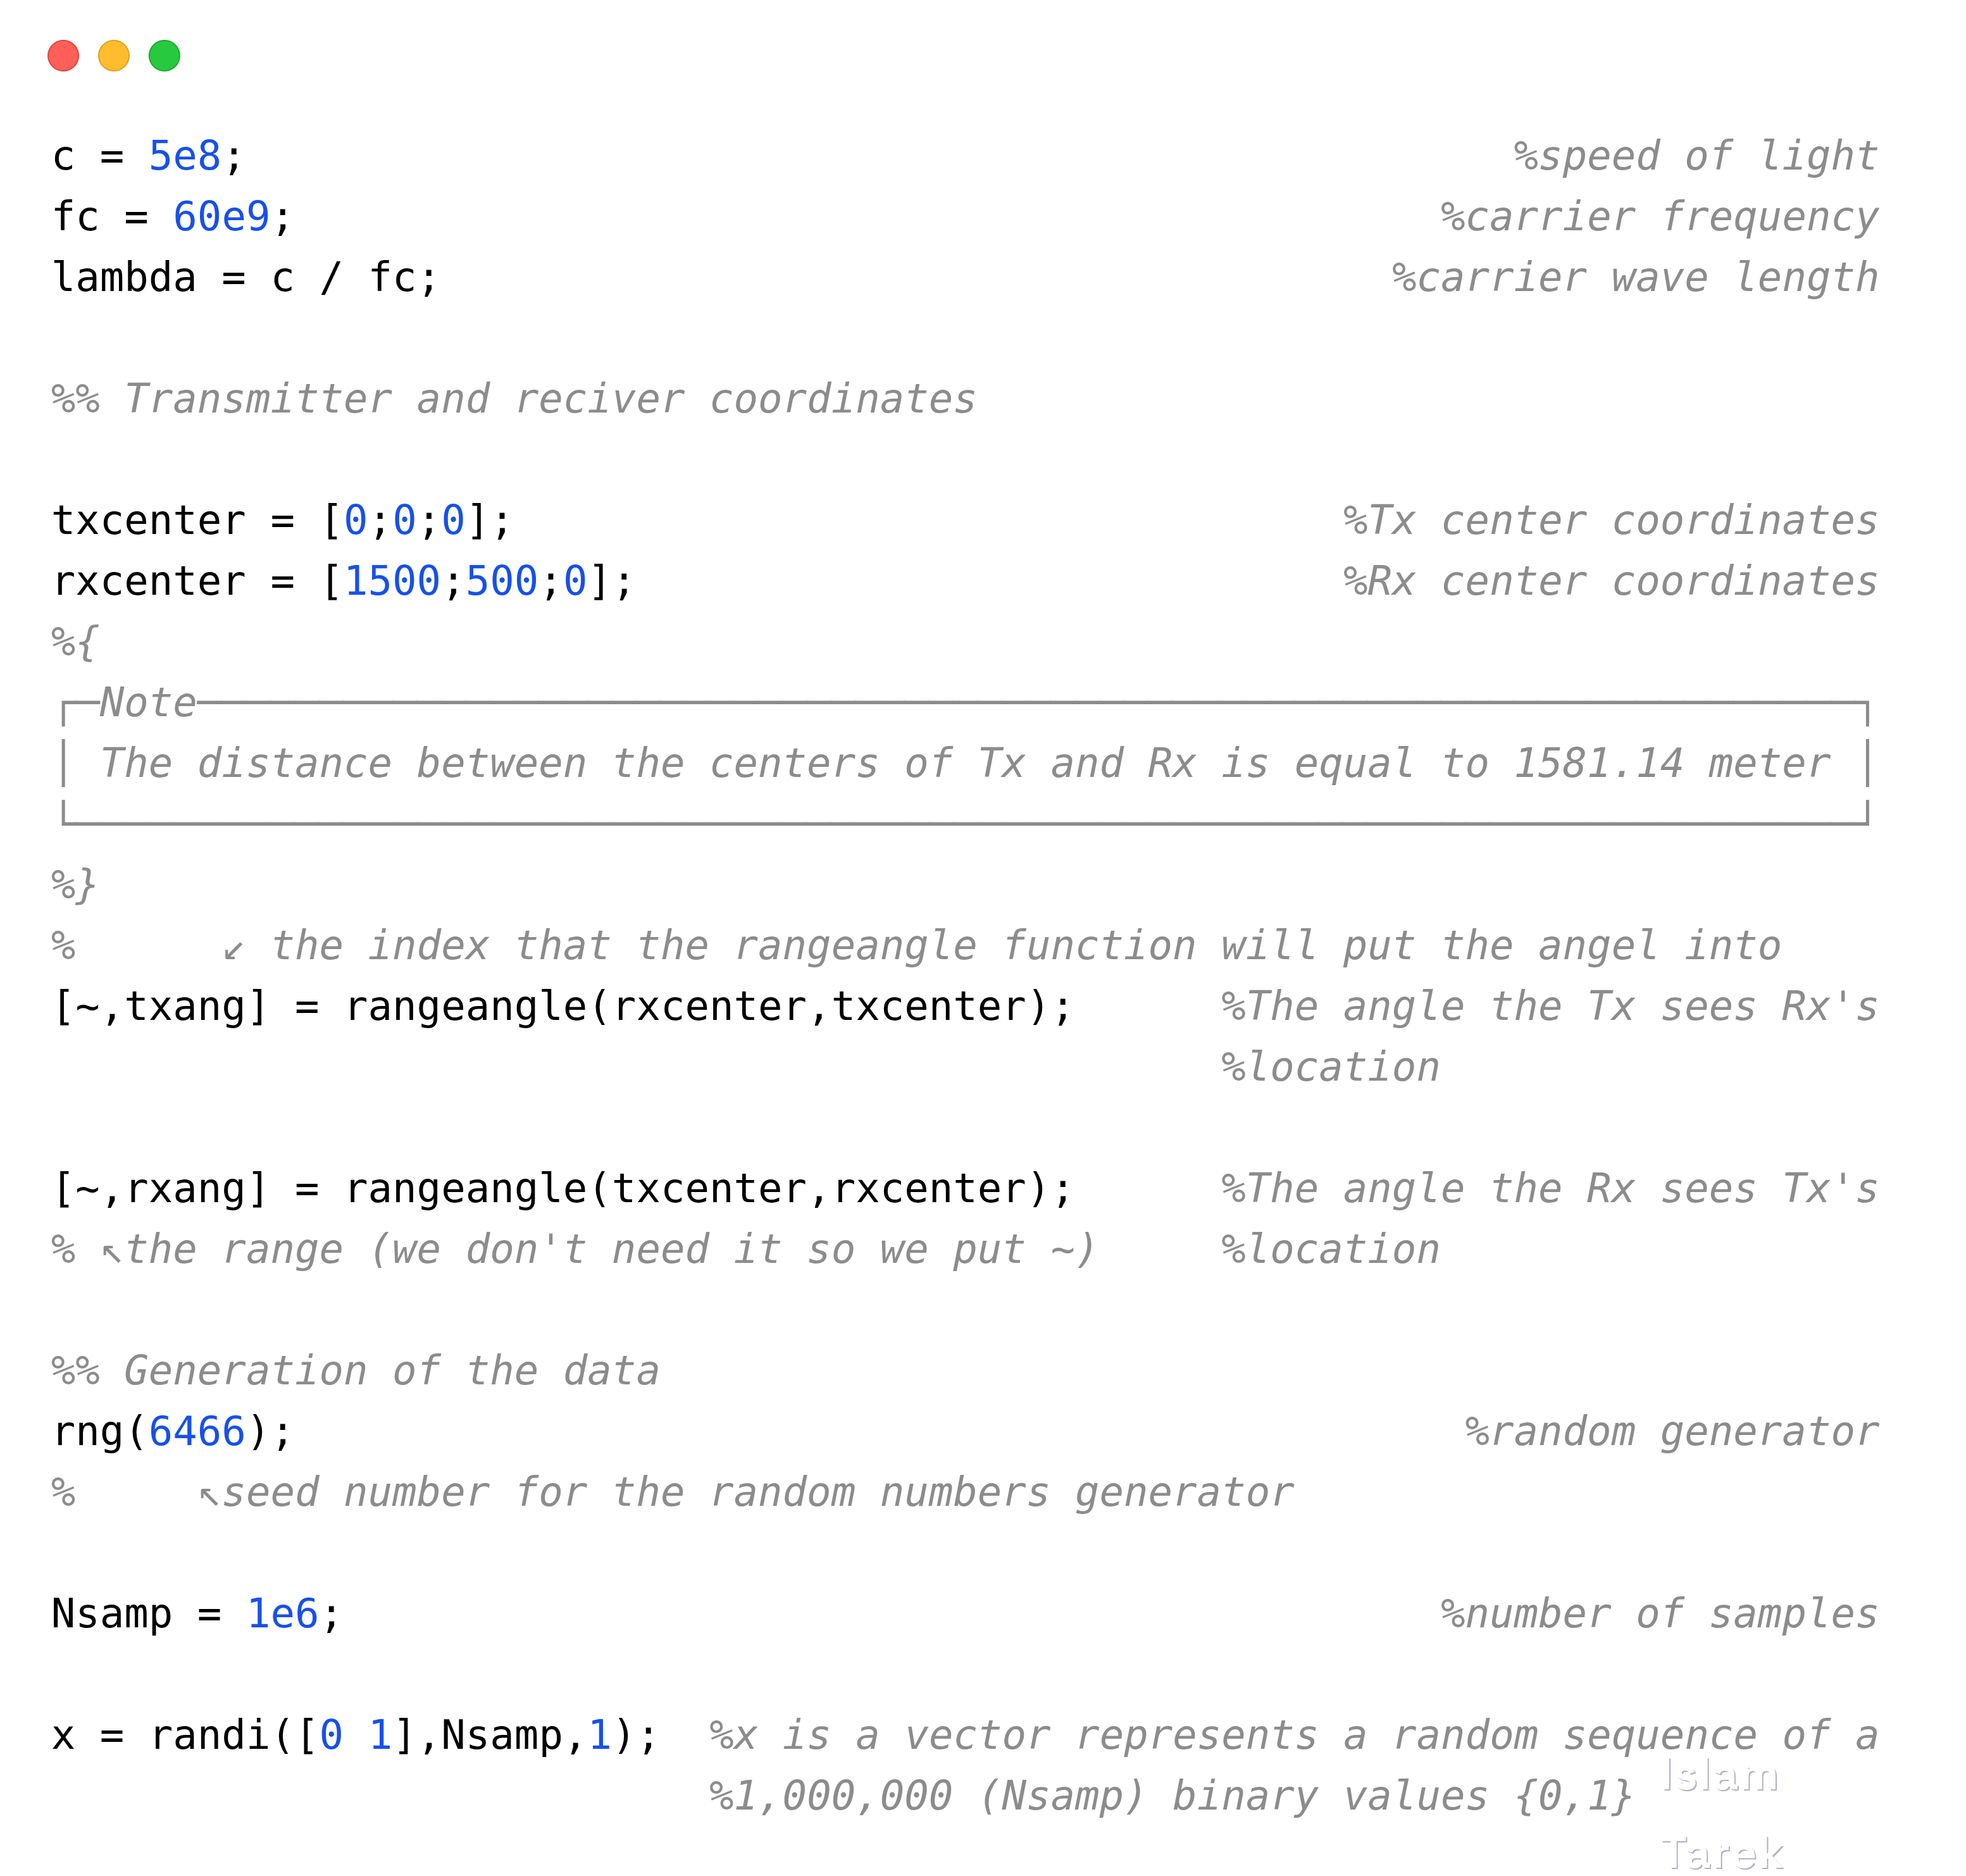
\includegraphics[width=0.8\linewidth]{figures/code1}
\end{figure}
\vfill
\restoregeometry